\documentclass[11pt, a4paper]{article}

\usepackage{amsmath, amssymb, titling}
\usepackage[margin=2.5cm]{geometry}
\usepackage[colorlinks=true, linkcolor=black, urlcolor=black, citecolor=black]{hyperref}
\usepackage{graphicx}
\usepackage{caption}
\usepackage{subcaption}
\usepackage{float}
\usepackage{cancel}
\usepackage{fancyhdr, lastpage}
\usepackage{fourier-orns}
\usepackage{xcolor}
\usepackage{nomencl}
\makenomenclature
\usepackage{etoolbox}
\usepackage{sidecap}
\usepackage{adjustbox}

\sidecaptionvpos{figure}{c}
\setlength{\headheight}{18.2pt}
\setlength{\nomlabelwidth}{1.5cm}

% \renewcommand\maketitlehooka{\null\mbox{}\vfill}
% \renewcommand\maketitlehookd{\vfill\null}

\renewcommand{\headrule}{\vspace{-5pt}\hrulefill\raisebox{-2.1pt}{\quad\leafleft\decoone\leafright\quad}\hrulefill}
\newcommand{\parder}[2]{\frac{\partial {#1}}{\partial {#2}}}
% \renewcommand\nomgroup[1]{%
%   \item[\bfseries
%   \ifstrequal{#1}{F}{Far--Away Properties}{%
%   \ifstrequal{#1}{N}{Dimensionless Numbers}{%
%   \ifstrequal{#1}{M}{Matrices}{%
%   \ifstrequal{#1}{D}{Diagonals}{%
%   \ifstrequal{#1}{V}{Vectors}{%
%   \ifstrequal{#1}{P}{Dimensionless Average Properties}{}}}}}}
% ]}

\title{Numerical Methods in Aeronautical Engineering \\ HW1}
\author{Almog Dobrescu ID 214254252}

% \pagestyle{fancy}
\cfoot{Page \thepage\ of \pageref{LastPage}}

\begin{document}

\thispagestyle{empty}
\begin{figure}[H]
    \centering
    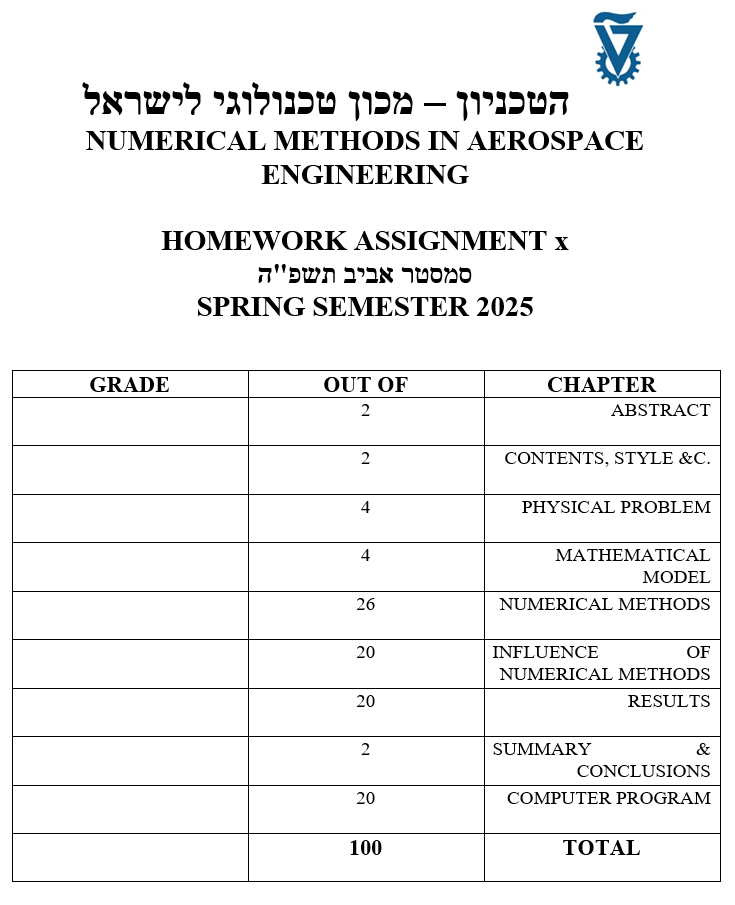
\includegraphics[width=\textwidth]{./../../../Cover page for computational assignments 2025.png}
    \label{fig: cover page}
\end{figure}
% \maketitle
\begin{center}
    \Huge
    Almog Dobrescu \qquad ID 214254252 \\ \vspace{0.5cm}
    \today
\end{center}
\newpage

\pagenumbering{roman}
% \setcounter{page}{1}
\begin{abstract}
    hello
\end{abstract}

\tableofcontents
\vfil
\listoffigures
\newpage

\printnomenclature
\newpage

\pagestyle{fancy}
\pagenumbering{arabic}
\setcounter{page}{1}

\section{The Physical Problem}
The physical problem at hand is the location of the flame front which depends on the point at which the fuel spray evaporates.

\section{The Mathematical Model}
The evaporation front of fuel spray can be described by solving the following equations:
\begin{equation}
    \begin{array}{c}
        \displaystyle\frac{d^2T}{d\zeta^2}=\Lambda e^T\left(T_v-T_u+\alpha\beta-\frac{dT}{d\zeta}\right) \\\\
        \displaystyle m_d=\left(\alpha\beta\Lambda e^T\right)^{-1}\frac{d^2T}{d\zeta^2}
    \end{array}
    \label{eq: mathematical model}
\nomenclature{$x$}{spatial coordinate}
\nomenclature{$T$}{temperature}
\nomenclature{$m_d$}{mass fraction of liquid fuel in droplets}
\nomenclature{$T_v$}{vaporization temperature of the liquid fuel}
\nomenclature{$T_u$}{environment temperature of the liquid fuel upstream}
\nomenclature{$\Lambda$}{empirical constant of droplet vaporation}
\nomenclature{$\alpha$}{mass ratio between the liquid fuel and environment oxigen}
\nomenclature{$\beta$}{ratio between the latent heat of the liquid fuel and between the chemical reaction heat of liquid vapor with oxigen}
\end{equation}
The boundary condition of the problem:
\begin{equation}
    \begin{array}{lccl}
        \begin{matrix}
            \zeta\rightarrow-\infty: && m_d\rightarrow1 \\
            \zeta\rightarrow+\infty: && T\rightarrow\zeta\cdot\left(T_v-T_u+\alpha\beta\right)
        \end{matrix} &&& \begin{matrix}
            T & \rightarrow & \zeta\cdot\left(T_v-T_u\right) \\
            m_d & \rightarrow & 0
        \end{matrix}
    \end{array}
\end{equation}
\begin{itemize}
    \item According to the defenition of $T$: $\left.T\right|_{\zeta=0}=0$
\end{itemize}

\section{The Numerical Methods}
Eq.\ref{eq: mathematical model} can be rewrite as:
\begin{equation*}
    \displaystyle\frac{d^2T}{d\zeta^2}+\Lambda e^T\frac{dT}{d\zeta}-\Lambda e^T\left(T_v-T_u+\alpha\beta\right)=0
    \label{eq: the ode}
\end{equation*}
In our case:
\begin{itemize}
    \item $\infty$ is at around $30$
    \item $\Lambda=0.1$
    \item $T_v=0.203$
    \item $T_u=0.152$
    \item $\alpha\beta=0.0234$
\end{itemize}

\subsection{Finite Difference Method}
Using central difference we can write the difference equations:
\begin{equation}
    \begin{array}{lcl}
        \displaystyle\frac{T_{i+1}-2T_i+T_{i-1}}{h^2}+\Lambda e^{T_i}\frac{T_{i+1}-T_{i-1}}{2h}-\Lambda e^{T_i}\left(T_v-T_u+\alpha\beta\right)=0 & \begin{matrix}
            i=1,2,\cdots,N \\\\
            \displaystyle h=\frac{\left.\zeta\right|_{i=N+1}-\left.\zeta\right|_{i=0}}{N+1-0}
        \end{matrix} 
    \end{array}
    \nomenclature{$h$}{size of each cell in the domain}
    \nomenclature{$i$}{cell index}
    \nomenclature{$N$}{number of elements}
\end{equation}
We will use the 'point Jacobi' method:
\begin{enumerate}
    \item Set the filed with initial condition (linear interpolation).
    \item Calculate the temperature at index \emph{i} and time step \emph{n+1} from the previous time step:
    \begin{equation}
        \begin{matrix}
            \begin{array}{c}
                \Lambda e^{T_i^{\left(n+1\right)}}=\frac{\displaystyle-\frac{T_{i+1}^{\left(n\right)}-2T_i^{\left(n\right)}+T_{i-1}^{\left(n\right)}}{h^2}}{\displaystyle\frac{T_{i+1}^{\left(n\right)}-T_{i-1}^{\left(n\right)}}{2h}-\left(T_v-T_u+\alpha\beta\right)} \\\\
                \Downarrow \\\\
                T_i^{\left(n+1\right)}=\displaystyle\ln\left(\frac{1}{\Lambda}\frac{\displaystyle-\frac{T_{i+1}^{\left(n\right)}-2T_i^{\left(n\right)}+T_{i-1}^{\left(n\right)}}{h^2}}{\displaystyle\frac{T_{i+1}^{\left(n\right)}-T_{i-1}^{\left(n\right)}}{2h}-\left(T_v-T_u+\alpha\beta\right)}\right)
            \end{array} && i=1,2,\cdots,N
        \end{matrix}
    \end{equation}
    \item The solution is considered converged when:
    \begin{equation}
        \left|y_i^{n+1}-y_i^n\right|<\varepsilon \hspace{1cm} \forall i\in[1, n]
    \end{equation}
\end{enumerate}

\subsection{Shooting Method}
Let's rewrite Eq.\ref{eq: the ode} as a system of 2 ODE:
\begin{equation}
    \begin{matrix}
        \left\{\begin{array}{lcl}
            \displaystyle\frac{dT}{d\zeta} & = & s \\\\
            \displaystyle\frac{ds}{d\zeta} & = & -\Lambda e^Ts-\Lambda e^{T}\left(T_v-T_u+\alpha\beta\right)
        \end{array}\right. && \begin{array}{l}
            \left.T\right|_{\zeta\rightarrow-\infty}\rightarrow\zeta\cdot\left(T_v-T_u\right) \\\\
            \left.T\right|_{\zeta\rightarrow+\infty}\rightarrow\zeta\cdot\left(T_v-T_u+\alpha\beta\right)
        \end{array}
    \end{matrix}
    \nomenclature{$s$}{temporery variable}
\end{equation}
To solve the system of equations using the shooting method, we will guess $s_{(i=0)}^{(n)}$ and solve the system of equations using forward difference. Namely:
\nomenclature{\fbox{$\cdot$}$^{(n)}$}{value at time step n}
\begin{equation}
    \begin{matrix}
        \left\{\begin{array}{lcl}
            \displaystyle T_{i+1}^{(n)} & = & s_i^{(n)}\cdot h+T_i^{(n)} \\\\
            \displaystyle s_{i+1}^{(n)} & = & \left(-\Lambda e^{T_i^{(n)}}s_i^{(n)}-\Lambda e^{T_i^{(n)}}\left(T_v-T_u+\alpha\beta\right)\right)\cdot h+s_i^{(n)}
        \end{array}\right. & \begin{array}{l}
            s_{i=0}^n=s_0^n \\\\
            T_{i=0}^n=\zeta\cdot\left(T_v-T_u+\alpha\beta\right) \\\\
            i=0,1,\cdots,N
        \end{array}
    \end{matrix}
\end{equation}
To correct the guess of $s_{(i=0)}^{(n)}$, let's define:
\begin{equation}
    F_{\left(s_{(i=0)}\right)}=T^{(n)}_{(i=N+1)}-\left.T\right|_{\zeta\rightarrow+\infty}
\end{equation}
\begin{itemize}
    \item When $F=0$, the guess of $s_{(i=0)}^{(n)}$ is correct
\end{itemize}
The next guess of \emph{s} $s_{(i=0)}^{(n+1)}$ we will use a numerical method to find the root of an equation. Namely:
\begin{equation}
    s_{(i=0)}^{(n+1)}=s_{(i=0)}^{(n)}-F_{\left(s_{(i=0)}^{(n)}\right)}\cdot\frac{s_{(i=0)}^{(n)}-s_{(i=0)}^{(n-1)}}{F_{\left(s_{(i=0)}^{(n)}\right)}-F_{\left(s_{(i=0)}^{(n-1)}\right)}}
\end{equation}

\section{Influence of The Numerical Methods}

\section{Results and Discussion}

\section{Summary and Conclusion}

\newpage
\appendix
\section{Listing of The Computer Program}

\end{document}